% 独自のコマンド

% ■ アブストラクト
%  \begin{jabstract} 〜 \end{jabstract}  :日本語のアブストラクト
%  \begin{eabstract} 〜 \end{eabstract}  :英語のアブストラクト

% ■ 謝辞
%  \begin{acknowledgment} 〜 \end{acknowledgment}

% ■ 文献リスト
%  \begin{bib}[100] 〜 \end{bib}


\newif\ifjapanese

\japanesetrue  % 論文全体を日本語で書く(英語で書くならコメントアウト)

\ifjapanese
  %\documentclass[a4j,twoside,openright,11pt]{jreport} % 両面印刷の場合。余白を綴じ側に作って右起こし。
  \documentclass[a4j,11pt]{jreport}                  % 片面印刷の場合。
  \renewcommand{\bibname}{参考文献}
  \newcommand{\acknowledgmentname}{謝辞}
\else
  \documentclass[a4paper,11pt]{report}
  \newcommand{\acknowledgmentname}{Acknowledgment}
\fi
\usepackage{thesis}
\usepackage{ascmac}
\usepackage{graphicx}
\usepackage{multirow}
\usepackage{url}
\bibliographystyle{jplain}

%\bindermode  % バインダー用余白設定

% 日本語情報(必要なら)
\jclass  {卒業論文}                             % 論文種別
\jtitle    {センシングデータを可視化する\\フレームワークの作成とその利用法の提案}    % タイトル。改行する場合は\\を入れる
\juniv    {慶應義塾大学}                  % 大学名
\jfaculty  {環境情報学部環境情報学科}               % 学部、学科
\jauthor  {永倉 啓太}                       % 著者
\jhyear  {26}                                   % 平成○年度
\jsyear  {2014}                                 % 西暦○年度
\jkeyword  {センシングデータ、ビジュアルプログラミング、Linda、データ可視化}     % 論文のキーワード
\jproject{増井俊之研究会} %プロジェクト名
\jdate{2014年1月}

% 英語情報(必要なら)


\begin{document}

\ifjapanese
  \jmaketitle    % 表紙(日本語)
\else
  \emaketitle    % 表紙(英語)
\fi

% ■ アブストラクトの出力 ■
%	◆書式:
%		begin{jabstract}〜end{jabstract}	:日本語のアブストラクト
%		begin{eabstract}〜end{eabstract}	:英語のアブストラクト
%		※ 不要ならばコマンドごと消せば出力されない。



% 日本語のアブストラクト
\begin{jabstract}
  近年、高性能のセンサーと豊富なリソースにより、iPhoneなどの端末で個人でも簡単にセンシングデータを取得できるようになった。加速度、傾き、位置情報など、多くのデータがビッグデータとしてあふれている。多くのデータはそれぞれが価値を持っているがそれらのデータを簡単に利用するフレームワークが現段階では存在しない。
そこで本研究ではセンシングデータを可視化し、データを簡単に取り出して利用できるフレームワークを作成した。本研究ではLindaという分散型プログラミングができるフレーワークを拡張した形になっている。Lindaは様々な場所で様々なユーザーが取得したセンシングデータをWeb上に流し、誰でも共有して利用できるようにしている。それらのセンシングデータをより簡単に利用できるようにすることで多くのプロダクトが産まれる可能性が広がるだろう。
  また、本研究ではセンシングデータを物に結びつけてプッシュAPI化する実装となっている。センシングデータを物と結びつけることでよりモジュール化し、より直感的に再利用できるメリットがある。

\end{jabstract}



% 英語のアブストラクト
  % アブストラクト。要独自コマンド、include先参照のこと

\tableofcontents  % 目次
\listoffigures    % 表目次
\listoftables    % 図目次

\pagenumbering{arabic}

\chapter{序論}
\label{chap:introduction}
\section{背景}
近年、データのセンシングが簡単になり多くのセンシングデータがビッグデータとしてあふれている。iPhoneやAndroidなどのスマートフォン端末でも位置情報や加速度、傾きなどのデータを常にセンシングすることが出来る。それに伴い、これらのセンシングデータを利用したアプリケーションが出されたり、研究目的として利用されたりするようになった。

しかしながら、これらのセンサーデータを簡単に利用できるようなフレームワークが現状存在しておらずデータをとっても活用せずに終わりといったケースが多かった。使い捨てのデータになっているこれらのデータを活用しない手はないだろう。

また、センサーデータを利用するアプリケーションは多数存在するが、個人がそれらのデータを使っているシーンは少ない。これは個人利用のハードルが高いためだ。多くの場合、プログラミング手段を用いてセンシングデータにアクセスしている。

まずはセンシングデータを可視化することでエンドユーザーに知らせることが必要だ。次点としてセンシングデータを簡単に利用できるように支援する必要がある。

個人が簡単にセンシングデータを利用できるようにするだけでより便利な世の中になるのではないだろうか。

\section{目的}
世の中に氾濫しているセンシングによるビッグデータをより効果的に利用するためのフレームワークを作成する。

そのためにまずはセンシングデータを理解できる数値、文字に変換することが必要になってくる。可視化できていなければどんなデータが利用できるかわからないためだ。

センシングデータを利用するためのフレームワークを作成する。これまでプログラミングができないとセンシングデータを利用できないケースが多くあり課題だったため、プログラミングをせずに使える直感的で使いやすいインタフェースを目指した。GUIでの操作は[1]の研究にもあるようにプログラミングせずに操作する有用な手法であると考えた。

また、他人が作ったセンシングデータをさらに再利用して使えるような仕組み作りをし、汎用的に多くの場面で使えるように想定した。

\section{本文書の構成}
第\ref{chap:introduction}章では本研究の概要を書いた。

第\ref{chap:contents}章では研究内容を説明する。第\ref{chap:prototype}章ではプロトタイプの実装方法を解説する。第\ref{chap:consideration}章では考察を書く。最後に第\ref{chap:conclusion}章にて結論を書き本論文をしめることとする。添付として参考文献を追記する。
  % 本文1
\chapter{研究内容}
\label{chap:contents}

本章では、本研究の内容を説明する。

\section{システム概要}

本システムはセンシングデータを個人でも簡単に利用できるようにすることが目的だ。
そのためのフレームワークを作成し、センシングデータを可視化するという二つの軸をもってシステムを構成した。

以下にシステムの構成を示す。大枠として、Linda\footnote{http://linda.masuilab.org\\データをクラウド上で共有するためのフレームワーク。並列処理で同時に多くのクライアントを処理できる。}からサーバーがデータを取得し、クライアントのリクエストに応じて送信する。クライアントでの情報は随時データベースに保存する。

\begin{table}[htbp]
  \caption{システム構成}
  \label{tb:files}
  \begin{center}\begin{tabular}{c|l}
    \hline
    システム&概要\\\hline\hline
    {\tt Linda}&データ元。データストリームからデータを取得する。\\\hline
    {\tt サーバー}&Lindaからデータを取得し、クライアントからのリクエストが来たら送信する。\\\hline
    {\tt クライアント}&サーバーにデータを要求し、ビジュアルプログラミングのビューを提供する。\\\hline
    {\tt データベース}&サーバー、クライアントのデータを保存している。\\\hline
  \end{tabular}\end{center}
\end{table}

\section{データの可視化}
センサーデータを二つの方法で可視化した。

まず一つ目として点滅によるデータの受信だ。Lindaから送られてきたデータを受信するとブロックが青に変化し、元に戻る。(図\ref{fig:image01})
センシングデータを監視してすぐにデータの受信に気付くことができるというメリットがある。\\

\begin{figure}[htbp]
  \begin{minipage}{0.5\hsize}
    \begin{center}
      \fbox{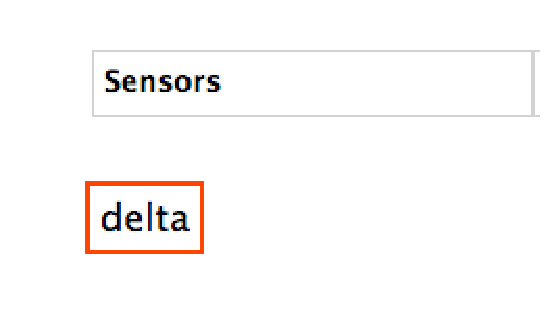
\includegraphics[width=50mm]{image/image1-1.eps}}
    \end{center}
  \end{minipage}
  \begin{minipage}{0.5\hsize}
    \begin{center}
      \fbox{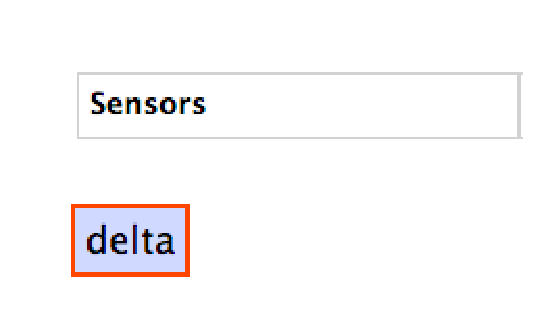
\includegraphics[width=50mm]{image/image1-2.eps}}
    \end{center}
  \end{minipage}
  \caption{点滅でのデータの通知}
  \label{fig:image01}
\end{figure}


そして二つ目として、実際の詳しいデータを見られるようにした。センサーオブジェクトに対してマウスオーバーしてフォーカスすることで実際の数字を表示できるようにした。(図\ref{fig:image02})

\begin{figure}[htbp]
    \begin{center}
       \fbox{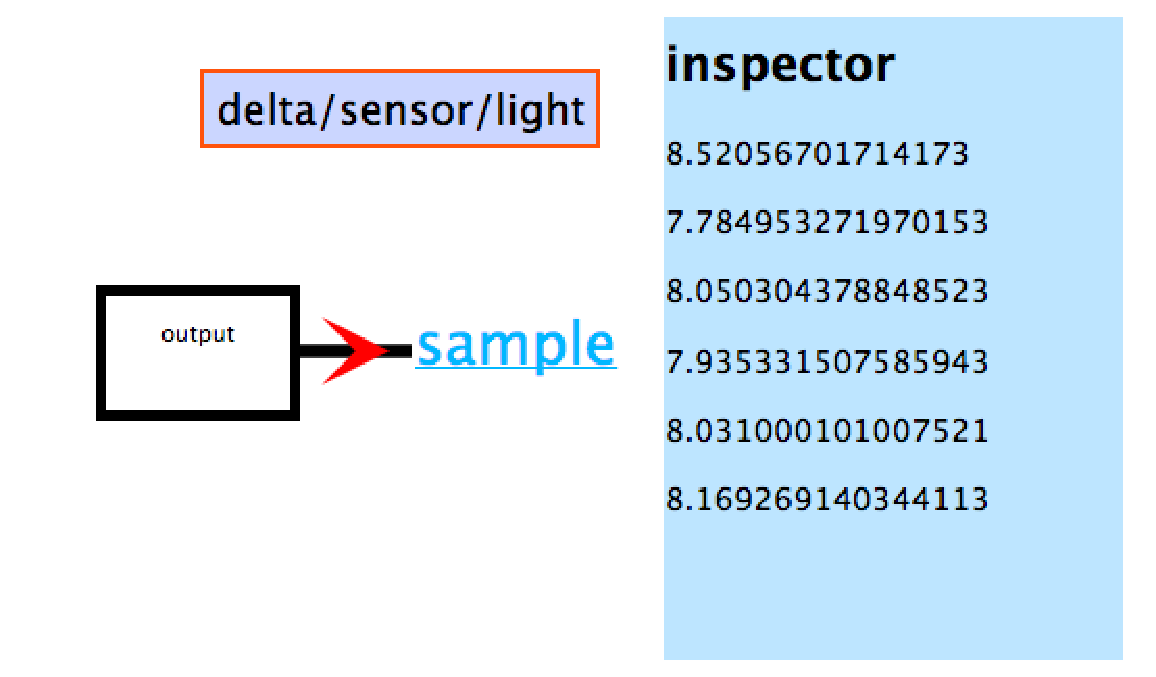
\includegraphics[width=100mm]{image/image02.eps}}
    \end{center}
    \caption{マウスオーバーによるデータの表示}
    \label{fig:image02}
\end{figure}

これら二つの実装により、センシングデータを閲覧する際に自分の欲しい粒度で取得することができるようになった。最低限の実装であれば詳しいデータが見られるだけでもいいが、抽象度を下げて色のみで表現することで閲覧する際の労力を下げることができる。

\section{ビジュアルプログラミング}

ビジュアルプログラミングを実装する際にブロック型のオブジェクトを作成した。以下にオブジェクトごとの解説をする。

\subsection{センサーオブジェクト}

ビジュアルプログラミングをする際には一番最初にセンサーオブジェクトを用意する。このオブジェクトはLindaからのデータを受信し、クライアント側でイベントを作成しデータを受信したら送信するというハブになっている。
また先に述べた通り、センサーデータが来るとこのブロックの点滅、あるいは能動的なデータの取得をすることが可能だ。

\subsection{条件オブジェクト}

センシングデータを扱うための条件オブジェクトを用意した。これにより上限下限、オンオフなどの条件分岐ができる。用意したオブジェクトを以下に列挙する。(図{\ref{fig:max}}〜図{\ref{fig:switch})これらのオブジェクトもブロックとして表現し、条件にマッチするとセンシングデータと同じように点滅する。

\begin{figure}[htbp]
  \begin{minipage}{0.5\hsize}
    \begin{center}
      \fbox{\includegraphics[width=50mm]{image/max.eps}}
    \end{center}
    \caption{Max: 最大値を設定}
    \label{fig:max}
  \end{minipage}
  \begin{minipage}{0.5\hsize}
    \begin{center}
      \fbox{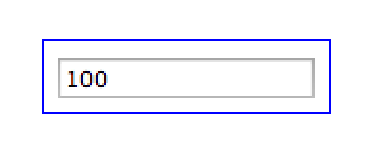
\includegraphics[width=50mm]{image/min.eps}}
    \end{center}
    \caption{min: 最小値を設定}
    \label{fig:min}
  \end{minipage}
\end{figure}

\begin{figure}[htbp]
  \begin{minipage}{0.5\hsize}
    \begin{center}
      \fbox{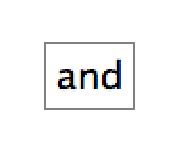
\includegraphics[width=50mm]{image/and.eps}}
    \end{center}
    \caption{and: 論理積を設定}
    \label{fig:and}
  \end{minipage}
  \begin{minipage}{0.5\hsize}
    \begin{center}
      \fbox{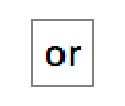
\includegraphics[width=50mm]{image/or.eps}}
    \end{center}
    \caption{or: 論理和を設定}
    \label{fig:or}
  \end{minipage}
\end{figure}

\begin{figure}[htbp]
  \begin{minipage}{0.5\hsize}
    \begin{center}
      \fbox{\includegraphics[width=50mm]{image/switch.eps}}
    \end{center}
    \caption{Switch: on/offを設定}
    \label{fig:switch}
  \end{minipage}
\end{figure}

\subsection{コネクションオブジェクト}

条件オブジェクトと同じ場所にあるが、その中で特殊なオブジェクトがコネクションオブジェクトである。コネクションオブジェクトはブロック間に親子件関係を作成できるオブジェクトである。

コネクションオブジェクトによって親のセンサーデータを条件オブジェクトの持つ自らの条件にかけ、次の世代に受け継ぐということが簡単にプログラムできるようになっている。

例えばdelta/sensor/lightからのセンサーデータかiota/sensor/lightからのセンサーデータがそれぞれ10以下でない場合にsampleというオブジェクトに通知を送るというような設定が簡単にできる。(図{\ref{fig:image03})

\begin{figure}[htbp]
    \begin{center}
       \fbox{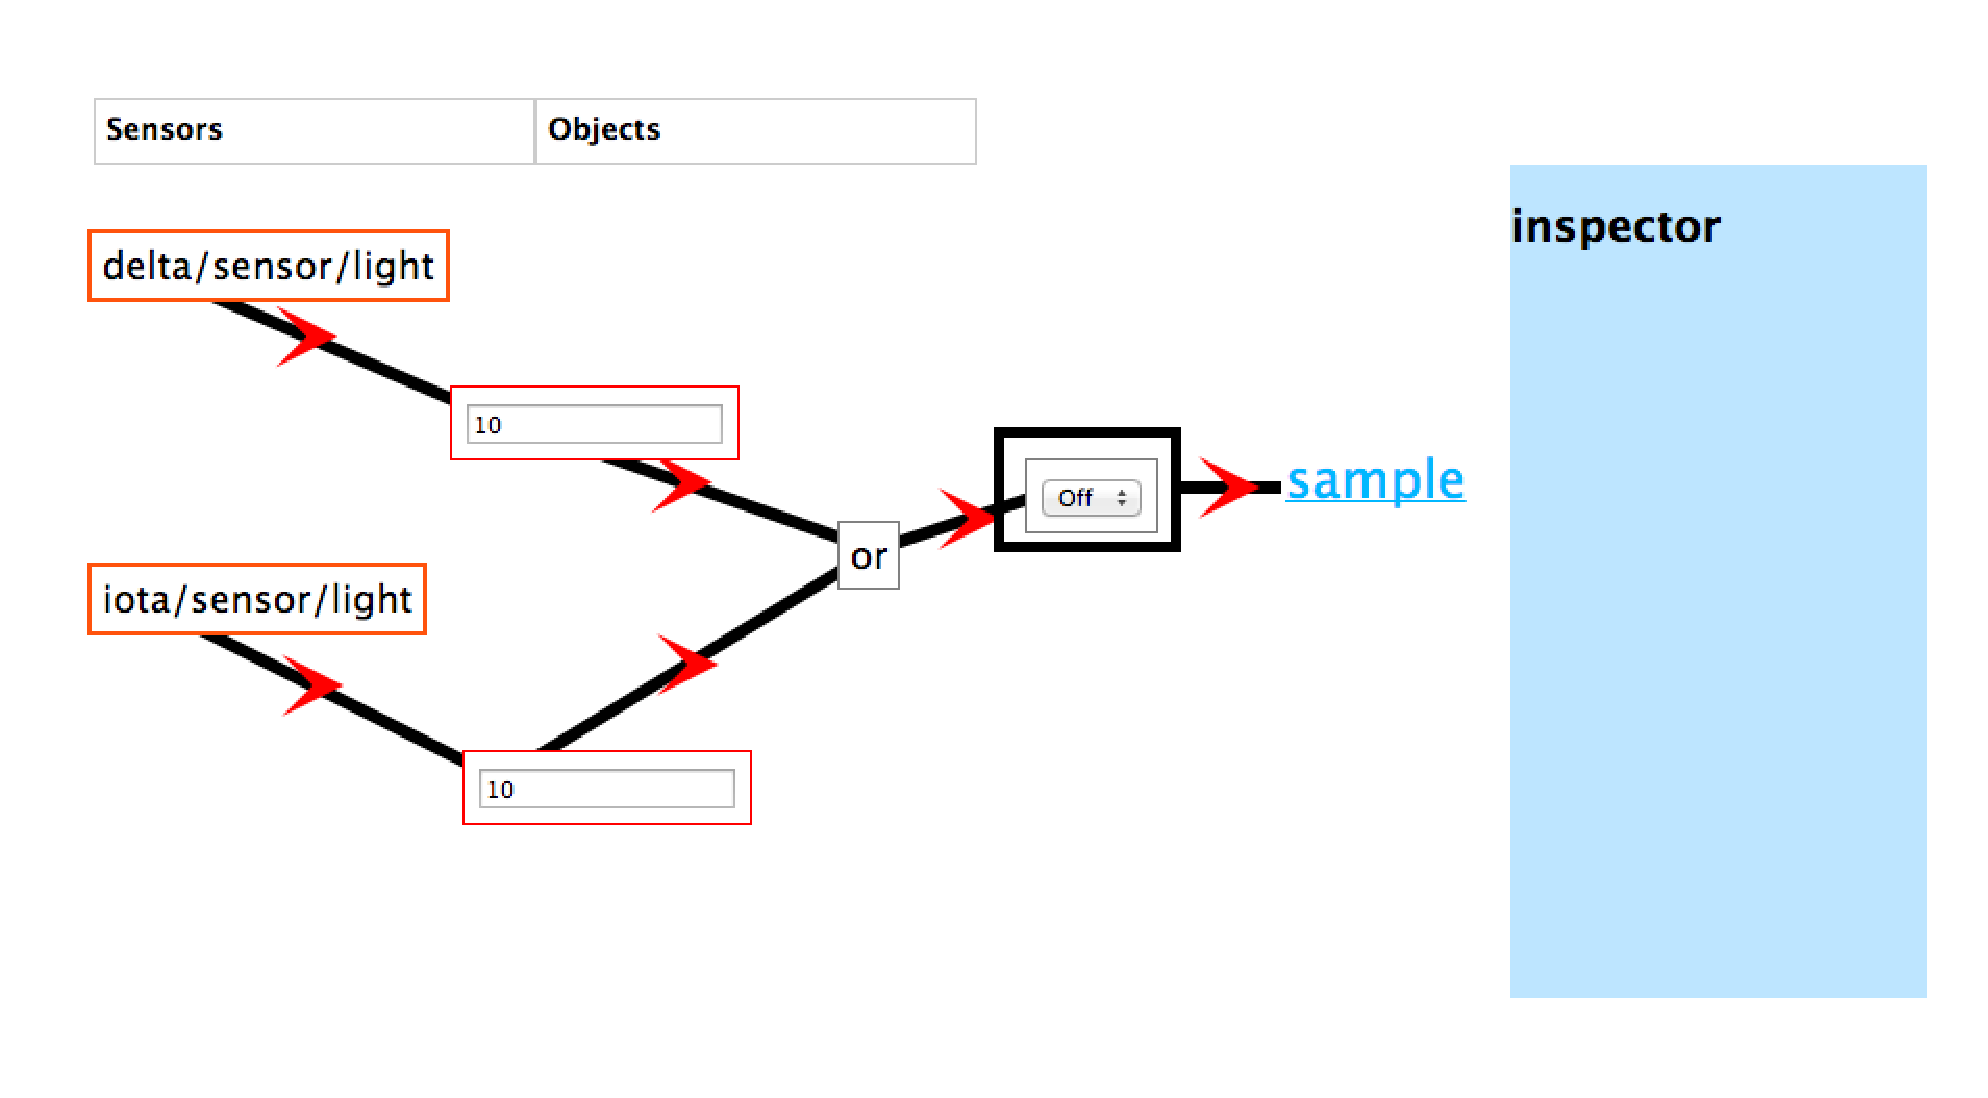
\includegraphics[width=150mm]{image/image03.eps}}
    \end{center}
    \caption{実際にセンシングデータをプログラミングする例}
    \label{fig:image03}
\end{figure}

\nocite{*}
  % 本文2
\chapter{プロトタイプの実装}
\label{chap:prototype}

この章では本研究でのプロトタイプを実装し、その流れを解説する。

\section{実装概要}
大量のデータをやりとりすることを想定してnode.js\footnote{http://www.nodejs.org/}で実装した。またデータベースはmongoDB\footnote{http://www.mongodb.org/}を採用し、軽量フレームワークを実現した。元になっているセンサーデータはLindaを利用し、データを取得、書き込みしている。

クライアントサイドではJQuery UI\footnote{http://jqueryui.com/}とSVG\footnote{http://www.w3.org/Graphics/SVG/}を使い、ドラッグ&ドロップと線の描画を実現している。

\section{ページ遷移}
パスによってページを管理している。基本的にはパスの名前が最終的に結びつけるオブジェクトの名前になっている。パスにアクセスした際、オブジェクトが作成されていなかった場合には新しいオブジェクトの作成が促され、データベースに記録される。ユーザーはそのオブジェクトに対してアクションとその条件を指定することでプログラムしていく。/keyというページに最初にアクセスした際にはkeyオブジェクトを作成する。最終的なアクションは/key/outputでPOST送信先を設定する。例えば部屋の明るさをセンシングし、部屋が暗くなったらという条件をkeyオブジェクトに紐付け、携帯に通知を送るというアクションを実行することなどができる。その他にも鍵の開け閉めをWebで管理している場合にはそのURLにリクエストを送ることもできる。

/controlのパスはデータベースの管理ができるようになっており、センサーやオブジェクトに追加が出来るようになっている。


\section{サーバーサイド}
言語はJavascriptを使い、node.jsのsocket.io\footnote{http://socket.io/}で実装した。センサーオブジェクトに対して常にコネクションを貼り、データをemitしている。mongoDBではセンサーデータ、オブジェクトデータ、コネクションデータ、クライアントデータを保存している。

\section{クライアントサイド}
クライアントサイドもサーバーサイドと同様にJavascriptを選択した。ページ内でオブジェクトの作成、移動、コネクションの作成などのアクションが行われた際に常にサーバー側に情報を送り保存している。イベントの制御にはEvent Emitter\footnote{http://nodejs.org/api/events.html}を用いた。Event Emitterを使えばオブジェクト自体にイベントを持たせることができる。それぞれのオブジェクトが送られてきたデータを監視し、自分の持っている条件にマッチしたら自らが送信側になるという実装をしている。下の図ではdelta/sensor/lightというセンサーを親データとして、orというオブジェクトが監視して条件に照らし合わせマッチしたら発信するオブジェクトになっている。(図\ref{fig:image09})

\begin{figure}[htbp]
  \begin{center}
    \fbox{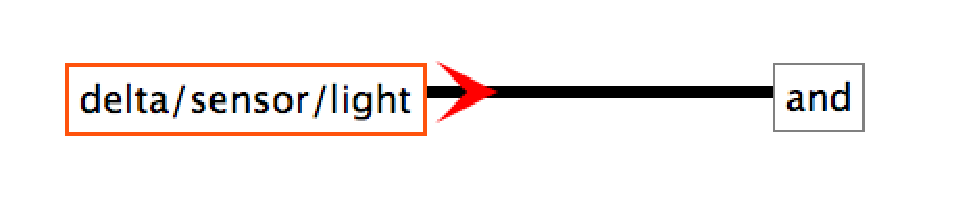
\includegraphics[width=100mm]{image/image09.eps}}
  \end{center}
  \caption{センサーデータの親子関係}
  \label{fig:image09}
\end{figure}

  % 本文3
\chapter{考察}
\label{chap:consideration}

この章では、よく使う\LaTeX のコマンドを説明する。足りない部分はぐぐればだいたいわかると思う。最初に書いておくと、数式を書く方法は、ぼく自身使わなかったので書いていない。ぼくのいた研究室でごりごり数式をたくさん書く必要のあるひとは、研究の種類からするとあまり居ない気がする。

\section{主なコマンド}

\subsection{章と節}

文書構造を明確にする大事なもの。目次はこれらのコマンドをもとに作られる。例えば、この第\ref{chap:latex}章の冒頭部分はこのようなソースで書かれている。

\begin{itembox}[l]{{\tt 03.tex}}
\begin{verbatim}
\chapter{\LaTeX の書き方}
\label{chap:latex}

この章では、よく使う\LaTeX のコマンドを説明する。(略)

\section{主なコマンド}

\subsection{章と節}

文書構造を明確にする大事なもの。目次はこれらのコマンドをもとに作られる。例えば、この第\ref{chap:latex}章の冒頭部分はこのようなソースで書かれている。
\end{verbatim}
\end{itembox}

章は \verb|\chapter{見出し}|、節は \verb|\section{見出し}|、小節は \verb|\subsection{見出し}|、小々節は \verb|\subsubsection{見出し}| を使う。表\ref{tb:chap}に一覧する。

\begin{table}[htbp]
  \caption{章と節のコマンド}
  \label{tb:chap}
  \begin{center}\begin{tabular}{c|c}
    \hline
    コマンド&用途\\\hline\hline
    \verb|\chapter{見出し}|&章\\\hline
    \verb|\section{見出し}|&節\\\hline
    \verb|\subsection{見出し}|&小節\\\hline
    \verb|\subsubsection{見出し}|&小々節\\\hline
    \end{tabular}\end{center}
\end{table}

\subsubsection{小々節見出しサンプルその1}

小々節は上のように \verb|\subsubsection{タイトル}| で書けるけれど、あまり文書の階層構造が深いことは望ましくないので、多用しなければならないようなら文書構造を見直したほうがよいと思う。

\subsubsection{小々節見出しサンプルその2}

小々節は、章や節、小節のように {\tt N.N.N} といった番号ではなくて、括弧付きの番号で出力される。かつ、目次には出力されない。

\subsection{図}

図は次のように出力される(図\ref{fig:sample1})。

\begin{figure}[htbp]
    \begin{center}
       \fbox{\includegraphics[width=50mm]{image.eps}}
    \end{center}
    \caption{図の例}
    \label{fig:sample1}
\end{figure}

ソースでは次のように記述している。

\begin{itembox}[l]{{\tt 03.tex}}
\begin{verbatim}
図は次のように出力される(図\ref{fig:sample1})。

\begin{figure}[htbp]
    \begin{center}
       \fbox{\includegraphics[width=40mm]{image.eps}}
    \end{center}
    \caption{図の例}
    \label{fig:sample1}
\end{figure}
\end{verbatim}
\end{itembox}

\verb|\begin{figure}[htbp]|  の{\tt htbp}は、表示位置の優先順位の設定。基本的に\LaTeX では、図の挿入位置は強制的には指定できない。いくつか候補を指定しておくと、候補のなかの優先度の高い順に、図を入れられるスペースがあるかどうかを調べて、入れられればそこに、入れられなければ次の候補のスペースを調べる、という処理が行われる。{\tt h}はこのコマンドを書いたその場所に、{\tt t}はページの一番上に、{\tt b}はページの一番下に、{\tt p}は画像だけ別ページに、それぞれ配置する。基本的には{\tt htbp}のように全部書いておけば問題ない。

\verb|\includegraphics| コマンドで、図のサイズと挿入するファイルを指定する。上の例ではサイズは {\tt width=50mm} として幅を指定したけれど、ここは他にも {\tt height=30mm} として高さを指定してもよいし、{\tt scale=0.5} として拡大率を指定してもよい。画像は最近の \LaTeX 環境であれば{\tt *.eps}以外でも使える。ただし、{\tt bb} (Bounding Box) として画像の大きさを指定する必要があることも多い。
以下はJPEG画像を使用する例。

\begin{itembox}[l]{{\tt 03.tex}}
\begin{verbatim}
\begin{figure}[htbp]
    \begin{center}
       \fbox{\includegraphics[width=40mm,bb=0 0 640 480]{image.jpg}}
    \end{center}
    \caption{図の例}
    \label{fig:sample1}
\end{figure}
\end{verbatim}
\end{itembox}

bbの指定は、上記のように{\tt *.tex} ファイルの中で指定してもいいが、
{\tt *.bb}ファイルを作っておく方法もある。
ターミナルで{\tt ebb}コマンドを使用すると{\tt *.bb}ファイルを簡単に作れる。


\begin{itembox}[l]{ebbコマンドの例}
\begin{verbatim}
% ebb image.jpg
\end{verbatim}
\end{itembox}


\verb|\includegraphics| を \verb|\fbox| に入れると、画像に枠を付けられる。

\verb|\caption| コマンドで図の見出しを指定できる。図の見出しは、図の下に表記するので注意。ここで指定した見出しが、図の目次に表示される。

\verb|\label| コマンドでは図の参照用ラベルを設定できる。本文中、\verb|\ref| コマンドで参照用ラベルを指定すると、対応した図の番号が自動的に挿入される。これも目次や参考文献と同様、最低二回のコンパイルが必要なので注意。

図を二つ横に並べたい場合は、次のように書く(図\ref{fig:sample2}、図\ref{fig:sample3})。

\begin{figure}[htbp]
  \begin{minipage}{0.5\hsize}
    \begin{center}
       \fbox{\includegraphics[width=40mm]{image.eps}}
    \end{center}
    \caption{図を並べる例1}
    \label{fig:sample2}
  \end{minipage}
  \begin{minipage}{0.5\hsize}
    \begin{center}
       \includegraphics[width=40mm]{image.eps}
    \end{center}
    \caption{図を並べる例2、枠なし}
    \label{fig:sample3}
  \end{minipage}
\end{figure}

\begin{itembox}[l]{{\tt 03.tex}}
\begin{verbatim}
図を二つ横に並べたい場合は、次のように書く(図\ref{fig:sample2}、図\ref{fig:sample3})。

\begin{figure}[htbp]
  \begin{minipage}{0.5\hsize}
    \begin{center}
       \fbox{\includegraphics[width=40mm]{image.eps}}
    \end{center}
    \caption{図を並べる例1}
    \label{fig:sample2}
  \end{minipage}
  \begin{minipage}{0.5\hsize}
    \begin{center}
       \fbox{\includegraphics[width=40mm]{image.eps}}
    \end{center}
    \caption{図を並べる例2}
    \label{fig:sample3}
  \end{minipage}
\end{figure}
\end{verbatim}
\end{itembox}


\subsection{表}

表は次のように出力される(表\ref{tb:sample1})。

\begin{table}[htbp]
  \caption{表の例}
  \label{tb:sample1}
  \begin{center}
  \begin{tabular}{l|c|r}
    \hline
    種類	&味&評価\\\hline\hline
    ドラ焼き&甘い&好き\\\hline
    メロンパン&カリもふ&好き\\\hline
    クリームパン&神&すごく好き\\\hline
  \end{tabular}\end{center}
\end{table}

ソースでは次のようになっている。

\begin{itembox}[l]{{\tt 03.tex}}
\begin{verbatim}
表は次のように出力される(表\ref{tb:sample1})。

\begin{table}[htbp]
  \caption{表の例}
  \label{tb:sample1}
  \begin{center}
  \begin{tabular}{l|c|r}
    \hline
    種類	&味&評価\\\hline\hline
    ドラ焼き&甘い&好き\\\hline
    メロンパン&カリもふ&好き\\\hline
    クリームパン&神&すごく好き\\\hline
  \end{tabular}\end{center}
\end{table}
\end{verbatim}
\end{itembox}

{\tt htbp}や \verb|\caption| と \verb|\label| は図と同様。ただし表のタイトルは表の上に書く。

\verb|\begin{tabular}{l|{\tt \textbar}{\tt c}{\tt \textbar}\verb|r}|で横方向のセルを指定する。{\tt c}は中央揃え、{\tt l}は左揃え、{\tt r}は右揃えのセルを作る。{\tt \textbar}は垂直方向の罫線を表す。{\tt c}か{\tt l}か{\tt r}を必要なセルの数だけ並べて、セルの間に罫線が必要なら{\tt \textbar}を入れればよい。

セルの中の文字は、{\tt \&}で区切って並べる。行と行は \verb|\\| で区切る。水平方向の罫線が必要なら、\verb|\hline| を書く。

水平方向や垂直方向のセルの結合もできる。例を示すので、くわしくはぐぐろう。説明がめんどう。\verb|\multirow|、\verb|\multicolumn|、\verb|\cline| を使うとできる。

\begin{table}[htbp]
  \caption{セルを結合した例}
  \label{tb:sample2}
  \begin{center}
  \begin{tabular}{c|c|c}
    \hline
    ほげ&ふー&ばー\\\hline\hline
    \multirow{2}{*}{ほげほげ}&\multicolumn{2}{c}{ふーふー} \\\cline{2-3}
    &ふーふーふー&ばーばーばー\\\hline
  \end{tabular}
  \end{center}
\end{table}

\begin{itembox}[l]{{\tt 03.tex}}
\begin{verbatim}
\begin{table}[htbp]
  \caption{セルを結合した例}
  \label{tb:sample2}
  \begin{center}
  \begin{tabular}{c|c|c}
    \hline
    ほげ&ふー&ばー\\\hline\hline
    \multirow{2}{*}{ほげほげ}&\multicolumn{2}{c}{ふーふー} \\\cline{2-3}
    &ふーふーふー&ばーばーばー\\\hline
  \end{tabular}
  \end{center}
\end{table}
\end{verbatim}
\end{itembox}


\subsection{脚注}

脚注は \verb|\footnote| コマンドを使う。例えばこんな感じ\footnote{ページの下に小さく説明を出せる}。

\begin{itembox}[l]{{\tt 03.tex}}
\begin{verbatim}
例えばこんな感じ\footnote{ページの下に小さく説明を出せる}。
\end{verbatim}
\end{itembox}

\section{その他のコマンド}

ぐぐる\footnote{http://www.google.co.jp/}。

特殊なことは何もしていないテンプレートなので、ぐぐって出たことはだいたいそのまま何でも使える。

あるいは、このファイル自体も\LaTeX で書かれているわけだから、これの{\tt *.tex}を見るのもよいかもしれない。


  % 本文4
\chapter{結論}
\label{chap:conclusion}

この章では、結論らしいことをかく。

\section{まとめ}

\LaTeX の環境さえあればスタンダードな体裁の論文がたぶんだれでも作れる程度のテンプレートにはなっているはず。がんばって卒業しよう。


\section{大事なこと}

箇条書きで列挙する。

\begin{itemize}
 \item ぐぐる。これは単なる\LaTeX だし、\LaTeX はもう枯れた技術だから、調べれば文献はいくらでもある。
 \item 先生を頼る。
 \item 単位をきちんとる。
 \item 卒業する。
\end{itemize}


  % 本文5

\begin{acknowledgment}
本研究を進めるにあたり、ご指導くださった増井俊之先生に深く感謝いたします。
アイデアの出し方、研究の進め方、実装方法など多くのことを学ばせていただきました。

橋本翔氏にはプログラミングの方法など、多くのことを学ばせて頂きました。ありがとうございました。

また、研究を進めるにあたり、増井研究室の皆様に多くのアドバイスを頂きました。心より感謝しております。\\\\
最後に学生生活を支えてくださった家族に感謝いたします。

\begin{flushright}
永倉 啓太
\end{flushright}

\end{acknowledgment}
  % 謝辞。要独自コマンド、include先参照のこと

\begin{bib}[100]
% BibTeXを使う場合
\bibliography{main}

%\begin{thebibliography}{#1}
%
%  \bibitem{参照用名称}
%    著者名:
%    \newblock 文献名,
%    \newblock 書誌情報,出版年.
%
% \bibitem{hoge09}
%   ほげ山太郎,ほげ山次郎:
%   \newblock ほげほげ理論のHCI分野への応用,
%   \newblock ほげほげ学会論文誌,Vol.31,No.3,pp.194-201,2009.
%
% \bibitem{hoge08}
%   Taro Hogeyama, Jiro Hogeyama:
%   \newblock The Theory of Hoge,
%   \newblock {\it The Proceedings of The Hoge Society}, 2008.
%
%\end{thebibliography}

\end{bib}
  % 参考文献。要独自コマンド、include先参照のこと
\appendix
\include{92_appendix}    % 付録

\end{document}
